\documentclass[tikz,border=12pt]{standalone}
\usepackage{amsmath,amssymb}
\usetikzlibrary{positioning,arrows,shapes,calc,backgrounds}

\begin{document}
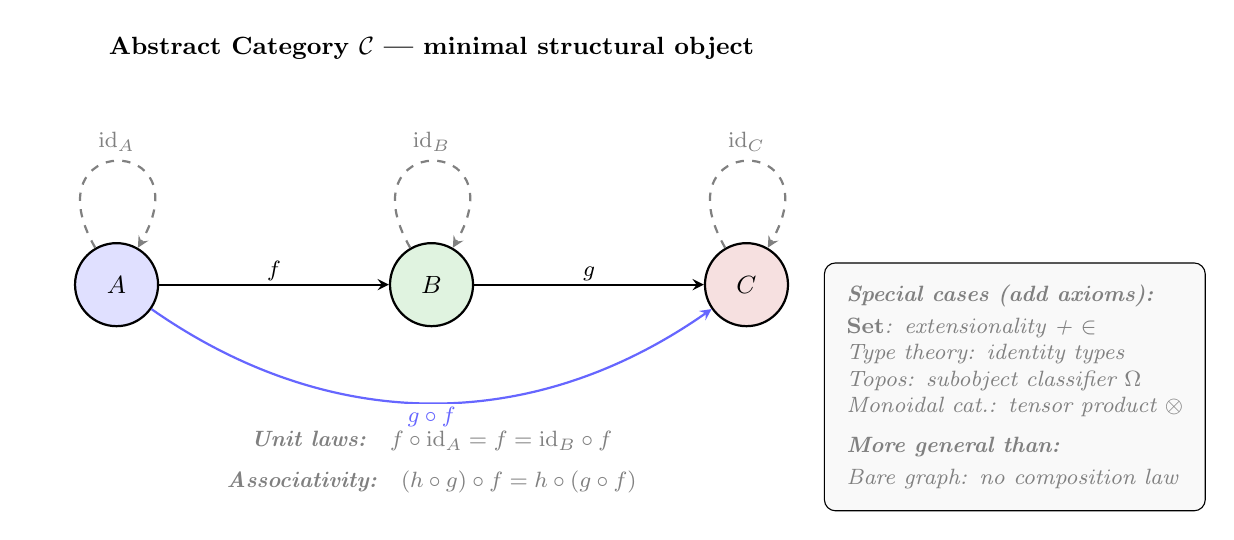
\begin{tikzpicture}[
  obj/.style={circle,draw,thick,fill=#1!12,minimum size=30pt,inner sep=0pt,font=\small\bfseries},
  mor/.style={->,>=stealth,thick},
  label/.style={font=\footnotesize,fill=white,inner sep=1pt},
  ann/.style={font=\footnotesize\itshape,text=gray,align=left},
]

% === Objects ===
\node[obj=blue] (A) at (0,0) {$A$};
\node[obj=green!60!black] (B) at (4,0) {$B$};
\node[obj=red!70!black] (C) at (8,0) {$C$};

% === Morphisms ===
\draw[mor] (A) -- node[label,above] {$f$} (B);
\draw[mor] (B) -- node[label,above] {$g$} (C);

% === Composition (curved below) ===
\draw[mor,bend right=35,blue!60] (A) to node[label,below] {$g \circ f$} (C);

% === Identity loops (dashed) ===
\draw[->,>=stealth,thick,dashed,gray] (A) edge[out=120,in=60,loop,looseness=8]
  node[above,font=\footnotesize] {$\mathrm{id}_A$} (A);
\draw[->,>=stealth,thick,dashed,gray] (B) edge[out=120,in=60,loop,looseness=8]
  node[above,font=\footnotesize] {$\mathrm{id}_B$} (B);
\draw[->,>=stealth,thick,dashed,gray] (C) edge[out=120,in=60,loop,looseness=8]
  node[above,font=\footnotesize] {$\mathrm{id}_C$} (C);

% === Title ===
\node[font=\small\bfseries,above=2.2cm of B] {Abstract Category $\mathcal{C}$ --- minimal structural object};

% === Axioms ===
\node[ann,below=1.2cm of B,align=center] {
\textbf{Unit laws:}\quad $f \circ \mathrm{id}_A = f = \mathrm{id}_B \circ f$\\[5pt]
\textbf{Associativity:}\quad $(h \circ g) \circ f = h \circ (g \circ f)$
};

% === Subsumption box ===
\begin{scope}[on background layer]
\node[draw,rounded corners,fill=gray!5,inner sep=8pt,ann,anchor=north west]
  at ($(C.north east)+(0.6,-0.1)$) {
\textbf{Special cases (add axioms):}\\[2pt]
$\mathbf{Set}$:\enspace extensionality + $\in$\\
Type theory:\enspace identity types\\
Topos:\enspace subobject classifier $\Omega$\\
Monoidal cat.:\enspace tensor product $\otimes$\\[5pt]
\textbf{More general than:}\\[2pt]
Bare graph:\enspace no composition law
};
\end{scope}

\end{tikzpicture}
\end{document}
